\documentclass[12pt]{article}
\usepackage{graphicx}
\usepackage[colorlinks=true]{hyperref}

\hypersetup{pdfauthor={Richard Barnes (ORCID: 0000-0002-0204-6040)},%
            pdftitle={CDCD's CD \#2 File Descriptor \& Data Notes},%
%            pdfsubject={Whatever},%
%            pdfkeywords={disease dynamics, mad cow disease, BSE, transmissible spongiform encephalopathy, prion},%
            pdfproducer={LaTeX},%
            pdfcreator={pdfLaTeX}
}

\title{CDCD's CD \#2 File Descriptor \& Data Notes}
\author{Richard Barnes}

\begin{document}

\maketitle

\tableofcontents

\section{Data Types}
There are three integer types used in the CDCD data.
\begin{center}
\begin{tabular}{c | l}
Data Type & Explanation \\
\hline
CHARACTER & A one-byte ASCII character \\
STRING & A character array (without a ending null) \\
INTEGER & A two-byte two's complement integer representation
\end{tabular}
\end{center}

No geodesic reference for the longitude and latitude values in the CDCD data was specified.

\section{File Types}
On the CD2 CD-ROM there are three types of files. They are discussed in the following sections.

\subsection{Index Files}
In each index file there is one header record and for each station in the data file there is one data record.

Stations in the index file are not arranged in any particular order (they were originally in order by station number, but insertions and deletions may have changed that somewhat); since none of the districts have a large number of stations (most have less than 100), a sequential search is roughly as fast, or faster, than any other method, and certainly less of a bother to program.  Sequence of stations in the index file is the same as for the associated data file.

\subsubsection{Path and Name of Index File}
\textbf{d}:\textbackslash{}\textbf{DistNumFirst}\textbackslash{}Data.\textbf{DistNum}, where \textbf{d} is replaced with the letter of the drive containing the CD-ROM, \textbf{DistNumFirst} is replaced by the first digit of the district number, and \textbf{DistNum} is replaced by the district number.

\subsubsection{Index File Header Record}
\begin{center}
\begin{tabular}{l|l|l}
Field & Data Type & Count \\
\hline
ID & STRING & 4 \\
MaxLat & INTEGER & 1 \\
MinLat & INTEGER & 1 \\
MaxLong & INTEGER & 1 \\
MinLong & INTEGER & 1 \\
MaxElev & INTEGER & 1 \\
MinElev & INTEGER & 1 \\
EarliestYear & INTEGER & 1 \\
LatestYear & INTEGER & 1 \\
NumberOfStns & INTEGER & 1 \\
DistrictID & STRING & 3 \\
DistrictName & STRING & 42
\end{tabular}
\end{center}

\subsubsection{Index File header Record Explanation}
\begin{itemize}
\item \textbf{ID} is a 4-char field that identifies the data-file version being used; for this version it's always ``WWWW"
\item \textbf{MaxLat} is the maximum latitude of any station found in this district; it is an integer representation of the degrees of latitude multiplied by 100 and added to the minutes of latitude; all values are considered to be West; e.g., 103$^\circ$26'W is 10326.
\item \textbf{MinLat} is the minimum latitude of any station found in this district; format is the same as MaxLat
\item \textbf{MaxLong} is the maximum longitude of any station found in this district; it is an integer representation of the degrees of longitude multiplied by 100 and added to the minutes of longitude; all values are considered to be north; e.g., 45$^\circ$50'N is 4550
\item \textbf{MinLong} is the minimum longitude of any station found in this district; format is the same as MaxLong
\item \textbf{MaxElev} is an integer representation of the maximum elevation of any station in this district
\item \textbf{MinElev} is an integer representation of the minimum elevation of any station in this district
\item \textbf{EarliestYear} is an integer representation of the earliest year of data of any station in this district
\item \textbf{LatestYear} is an integer representation of the latest year of data of any station in this district
\item \textbf{NumberOfStns} is an integer representation of the number of stations in this district
\item \textbf{DistrictID} is the 3-character district number (e.g., ``101" to ``850")
\item \textbf{DistrictName} is the official name of the district  (e.g., ``Lower Saskatchewan River Basin"); 42 characters are reserved for this field
\end{itemize}

\subsubsection{Index File Data Record Structure}
\begin{center}
\begin{tabular}{l | l | l}
Field & Data Type & Count \\
\hline
CSN & STRING & 4 \\
StationName & STRING & 24 \\
Airport & STRING & 3 \\
Latitude & INTEGER & 1 \\
Longitude & INTEGER & 1 \\
Elevation & INTEGER & 1 \\
FirstYear & INTEGER & 7 \\
LastYear & INTEGER & 7 \\
StartingRecordNumber & INTEGER & 1
\end{tabular}
\end{center}

\subsubsection{Index File Data Record Explanation}
\begin{itemize}
\item \textbf{CSN} is the last four characters of the 7-character station ID (e.g., for ``6158733" this would contain ``8733")
\item \textbf{StationName} is the station's name as found in the Station Data Catalogues; 24 characters are reserved for this field
\item \textbf{Airport} is the three-character airport identifier that some stations have (e.g., ``YWG" for Winnipeg); if none exists for this station then the field is left blank
\item \textbf{Latitude} is an integer representation of the degrees of latitude multiplied by 100 and added to the minutes of latitude; all values are considered to be West; e.g., 103$^\circ$26'W is 10326
\item \textbf{Longitude} is an integer representation of the degrees of longitude multiplied by 100 and added to the minutes of longitude; all values are considered to be north; e.g., 45$^\circ$50'N is 4550
\item \textbf{Elevation} is the elevation in metres
\item \textbf{FirstYear} is a seven-integer array containing the first year of data for the station, and for each of the six elements (in the order 001,002,010,011,012,013)
\item \textbf{LastYear} is a seven-integer array containing the last year of data for the station, and for each of the six elements (in the order 001,002,010,011,012,013)
\item \textbf{StartingRecordNumber} is the record number of the first record for the station; this record is a header that contains information about the station
\end{itemize}

\subsection{STATIONS.ALL}
This file is found on the root directory.

This file contains all of the Index File Header records (in order); it's useful when compiling a list of districts and related information


\subsection{Data files}
In the data file each station begins with a header record, and then the station's data records (one record for one element for one year). The file contains one header record for each station.

\subsubsection{Path and Name of Data File}
\textbf{d}:\textbackslash{}\textbf{DistNumFirst}\textbackslash{}Data.\textbf{DistNum}, where \textbf{d} is replaced with the letter of the drive containing the CD-ROM, \textbf{DistNumFirst} is replaced by the first digit of the district number, and \textbf{DistNum} is replaced by the district number.

\subsubsection{Data File Header Record Structure}
\begin{center}
\begin{tabular}{l | l | l}
Field & Data Type & Count \\
\hline
ID & STRING & 4 \\
CSN & STRING & 7 \\
StationName & STRING & 24 \\
Airport & STRING & 3 \\
Latitude & INTEGER & 1 \\
Longitude & INTEGER & 1 \\
Elevation & INTEGER & 1 \\
FirstYear & INTEGER & 1 \\
LastYear & INTEGER & 1 \\
RecNumb & INTEGER & 300 \\
DataAvailable & CHARACTER & 300 \\
Filler & CHARACTER & 123
\end{tabular}
\end{center}

\subsubsection{Data File header Record Explanation}
\begin{itemize}
\item \textbf{ID} is a 4-char field that identifies the data-file version being used; for this version it's always ``WWWW"
\item \textbf{CSN} is the 7-character station ID as found in the station data catalogues (e.g., ``6139525")
\item \textbf{StationName} is the station's name as found in the Station Data Catalogues; 24 characters are reserved for this field
\item \textbf{Airport} is the three-character airport identifier that some stations have (e.g., ``YWG" for Winnipeg); if none exists for this station then the field is left blank
\item \textbf{Latitude} is an integer representation of the degrees of latitude multiplied by 100 and added to the minutes of latitude; all values are considered to be West; e.g., 103$^\circ$26'W is 10326
\item \textbf{Longitude} is an integer representation of the degrees of longitude multiplied by 100 and added to the minutes of longitude; all values are considered to be north; e.g., 45$^\circ$50'N is 4550
\item \textbf{Elevation} is the elevation in metres
\item \textbf{FirstYear} is an integer containing the first year of data for the station
\item \textbf{LastYear} is an integer containing the last year of data for the station
\item \textbf{RecNumb} is a 300-element integer containing the record number of each year's first element; this number is an offset from the header record (the first record following the header is record \#1); in this array the first element is for the year 1801, the 100th is for 1901, the 150th is for 1951, etc.
\item \textbf{DataAvailable} is a 300-element single-character element that contains information about the availability of data in a year. Each character in this array is a bit-field in which each of the right-most six bits indicates whether or not an element is available for a requested year; e.g., if the entire byte is ``00100011" this indicates that there is data for the first, second, and sixth elements.

From right to left, the elements indicated are:  Maximum Temperature (001), Minimum Temperature (002), One-Day Rainfall (010), One-Day Snowfall (011), One-Day Precipitation (012), Snow On The Ground (013).  As with the RecNumb array the first element is the year 1801, the 100th is for 1901, etc.

The elements' representation in the data file follows the order above.
\item \textbf{Filler} takes up 123--bytes and is only here to pad the record out to the same length as a data record (1071 bytes); fixed-length records make life easier when reading the file
\end{itemize}

\subsubsection{Data File Data Record Structure \& Explanation}
There is one basic format with several different variations, depending upon the element contained within. 

The structure is as follows:
\begin{itemize}
\item an array of 366 integer values (2 bytes each), each containing one day's value; 
\item an array of 366 flags (1 nibble each), each containing one day's flag. This array can be expanded to 366 bytes, in which each byte has a value between 0 and 15.  Flags corresponding to these values are (for notes on missing data be sure to see Section \ref{sec:missing}, below):
	\begin{center}
	\begin{tabular}{c | c | p{8cm}}
	Integer Value & Character & Explanation \\
	\hline
	0 & - & No Flag \\
	1 & E & Estimated\\
	2 & T & Trace occurred. Value is 0. \\
	3 & C & Precip occurred; amount is uncertain; recorded value is 0. \\
	4 & L & Precip may or may not have occurred; amount is unknown; recorded value is 0. \\
	5 & A & Amount accumulated over more than one day; previous value's flag was C or L. \\
	6 & F & Amount accumulated over more than one day and estimated \\
	\hline
	7 & - & Unused \\
	8 & - & Unused \\
	9 & - & Unused \\
	10 & - & Unused \\
	11 & - & Unused \\
	12 & - & Unused \\
	13 & - & Unused \\
	\hline
	14 & φ & (ASCII 237) This is used to denote February 29th in a non-leap year \\
	15 & M & Missing
	\end{tabular}
	\end{center}
\item 12 sets of summary values (each set 13 bytes in length) of monthly data for a total size of 12*13=156 bytes. In the following, variables that are marked as CHARACTER are actually single-byte integers; their ASCII value corresponds to their numeric value. Note that, except for Snow on the Ground, all values need to be divided by 10; e.g., the value 10.3 is stored as 103 (this is done to remove the need to store values as the more space-consuming floating-points).
\begin{itemize}
\item \textbf{Maximum Temperature} \\
\begin{tabular}{c | l | p{6cm}}
Number & Data Type & Explanation \\
\hline
1 & INTEGER & Mean Max for Month \\
2 & CHARACTER & \# Days Missing \\
3 & CHARACTER & \# Days With Max \textgreater 0C \\
4 & INTEGER & Maximum Max For Month \\
5 & CHARACTER & Date of Maximum Max \\
6 & INTEGER & Minimum Max for Month (this was listed as a character in the specification, but is more likely to be an integer) \\
7 & CHARACTER & Date of Minimum Max \\
8 & CHARACTER & Max \# Days in a Row with Missing Data \\
9 & CHARACTER & \# Days with Missing Mean Temp \\
10 & CHARACTER & Maximum \# Days in a Row with Missing Mean Temp
\end{tabular}

\item \textbf{Minimum Temperature} \\
\begin{tabular}{c | l | p{6cm}}
Number & Data Type & Explanation \\
\hline
1 & INTEGER & Mean Minimum for Month \\
2 & CHARACTER & \# Days Missing \\
3 & CHARACTER & \# Days with Min \textgreater 0C \\
4 & INTEGER & Maximum Min for Month \\
5 & CHARACTER & Date of Maximum Min \\
6 & CHARACTER & Minimum Min for Month \\
7 & CHARACTER & Date of Minimum Min \\
8 & CHARACTER & Max \# Days in a Row with Missing Data \\
9 & INTEGER & Mean Temperature
\end{tabular}

\item \textbf{Precipitation (Rain, Snow, Total Pcpn)} \\
\begin{tabular}{c | l | p{6cm}}
Number & Data Type & Explanation \\
\hline
1 & INTEGER & Total for Month \\
2 & CHARACTER & \# Days Missing \\
3 & CHARACTER & \# Days with \textgreater 0 cm/mm \\
4 & INTEGER & Max one-day total for Month \\
5 & CHARACTER & Date of Max \\
6 & CHARACTER & \# Days with \textgreater Trace \\
7 & CHARACTER & \# Days with \textgreater 1 cm \\
8 & CHARACTER & \# Days with Uncrtn/accum pcpn \\
9 & CHARACTER & Maximum \# Days in a row with Uncrtn/accum Pcpn \\
10 & CHARACTER * 2 & Unassigned
\end{tabular}
\item \textbf{Snow on the Ground} \\
\begin{tabular}{c | l | p{6cm}}
Number & Data Type & Explanation \\
\hline
1 & INTEGER & Median for Month \\
2 & CHARACTER & \# Days Missing \\
3 & CHARACTER & Days with \textgreater 0 cm \\
4 & INTEGER & Max for Month \\
5 & CHARACTER & Date of Max \\
6 & INTEGER & Min for Month \\
7 & CHARACTER & Date of Min \\
8 & CHARACTER & Days with \textgreater Trace \\
9 & CHARACTER & Days with \textgreater 1 cm \\
10 & CHARACTER * 2 & Unassigned
\end{tabular}
\end{itemize}
\end{itemize}

\section{Special Considerations Regarding Missing Data}
\label{sec:missing}
The value \textbf{-9999} in any field implies that that field is missing.

Accumulated values (those with the flags ``A" and ``F") are not used by the Extremes. When processing the Sums \& Averages section the following rules are used to decide whether months/seasons should be considered to be missing:
\begin{itemize}
\item a month of temperature data will be considered as missing when it has more than a total of five daily values missing or when there are more than three consecutive dail values missing at any point in the month
\item a month of precip data will be deemed as missing when it has any missing daily values (Note that while precip flags indicating accumulated values are always considered to be issing for the purposes of the extremes section, they only constitute a period of missing data in this section when there are mroe than four consectuvie days with an ``A", ``C", ``F", or ``L" flag. A season with any missing monthly values will be considered to be missing
\end{itemize}

\section{How To Obtain Data From the CD}
Following are the basic steps required to obtain data values from the CD.
\begin{enumerate}
\item Read index file for district
\begin{itemize}
\item sequentially seek through the index file until the required station is found (the largest index file is less than 16K, so this is not a lengthy procedure).
\item from the index file get the information about the station and its location.  Note that the location data is for the most part only ``nice to know" material, the FirstYear and LastYear arrays are useful by not absolutely essential, and the StartingRecordNumber is necessary if the reading software is not to do a sequential search through all stations preceding the requested station.
\end{itemize}
\item Read the station's header information found in the data file for the appropriate district
\begin{itemize}
\item The header record is found at the location pointed to by the value in StartingRecordNumber previously read from the index file
\end{itemize}
\item Using DataAvailable and RecNumb arrays determine whether or not data exists for a given year, and if so what the record number is for the first record in that year.
\item From the data file, read the data for the required year, convert daily flags, and any necessary monthly character/integer data.
\end{enumerate}

\begin{figure*}[h]
\centering
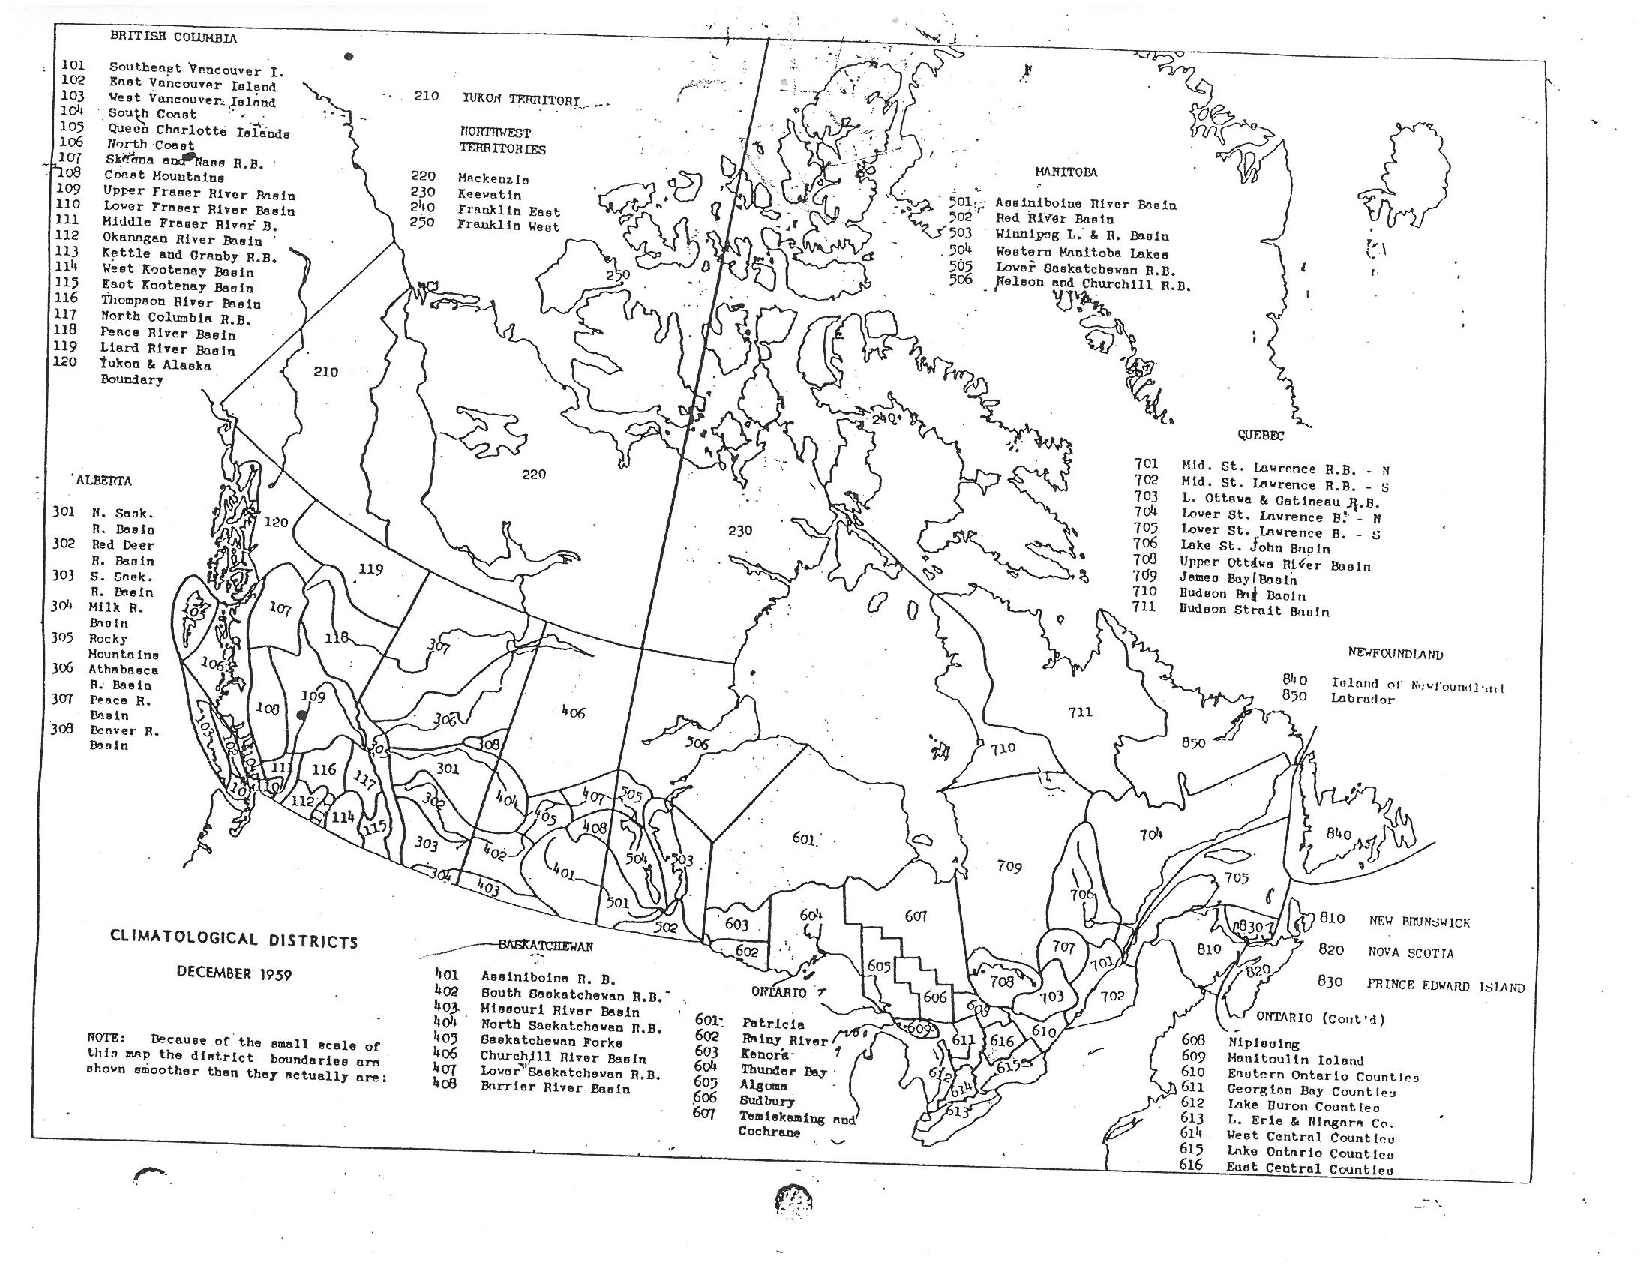
\includegraphics[width=\linewidth]{Climatological_Districts.pdf}
\caption{Climatological Districts of Canada (Picture Zooms Well)}
\end{figure*}

\section{Documentation History}
This document was compiled by Richard Barnes (barn0357@umn.edu) of the University of Minnesota during work on a project involving tracking the trajectories of intersections of fitted mathematical surfaces of climate data. The project was directed by Dr. Clarence Lehman (lehman@umn.edu), also of the University of Minnesota.

This document has been produced using materials provided by Climate Services, but they have not verified the accuracy of the information herein. Any mistakes in the information provided by this document were either original to the documentation provided by Climate Services or unintentionally introduced by the author (Richard Barnes). You use this document at your own risk. If you do find mistakes, please check the original documentation and contact either the author (Richard Barnes) and/or Climate Services, as appropriate.

The original CDCD data format specification was written in March, 1993 and was called ``CD2 File Formats"; it's file name was ``FILEINFO\_word.doc". It was provided to me in a personal communication with a member of the office listed below.

\begin{verbatim}
Weather and Environmental Monitoring 
Meteorological Service of Canada 
Environment Canada 
4905 Dufferin Street, Toronto, ON M3H 5T4 
Climate.Services@ec.gc.ca
\end{verbatim}

``FILEINFO\_word.doc" contained several errors, which I have corrected above. There were also omissions, such as the meaning of flags, an exact definition of data types, a note on the use of -9999 as a missing value indicator, and data selection strategies. Some of this information was gleaned by reading the User Guide inside the old DOS program the CDCD packages to decode their data. To be fair, this program is quite useful for browsing the data, but useless when it comes to mass-analysis.

Upon request, I was also provided the Climatological Map of Canada's climate districts, initially as an low-quality BMP named ``CXMAP.BMP" and then as a high-quality PDF named ``Climatological\_Districts.pdf". To my knowledge this map is not in any publically accessible archive.

The Climate Services technicians also offered to give me access to a repository of data used to generate the CDCD information, though that repository was not generally available to the public. The data format of this repository is much friendlier, being a long set of values of the format ``STATION YEAR MONTH DAY 1 DAY 2 DAY 3 ..."

\end{document}
